\documentclass[aps,prl,onecolumn,amsmath,amssymb,superscriptaddress]{revtex4-2}

\usepackage{bm}
\usepackage{booktabs}
\usepackage{graphicx}
\usepackage{microtype}
\usepackage{xcolor}
\usepackage[colorlinks=true,linkcolor=blue!50!black,citecolor=blue!50!black,urlcolor=blue!50!black]{hyperref}

\graphicspath{{figures/}}

\newcommand{\Jzz}{J_{zz}}
\newcommand{\Jpm}{J_{\pm}}
\newcommand{\ghex}{g_{\mathrm{hex}}}
\newcommand{\gfour}{g_4}
\newcommand{\bq}{\bm q}
\newcommand{\br}{\bm r}
\newcommand{\bdelta}{\bm\delta}
\newcommand{\btheta}{\bm\theta}
\newcommand{\ice}{\mathcal I}

\begin{document}

\title{Supplemental Material for ``Winding-Free Exact Diagonalization of Quantum Spin Ice''}
\author{Z.-B.~Zhou}
\affiliation{Department of Physics, [institution], [city], [country]}
\date{\today}
\maketitle

This Supplemental Material provides the FCC-32 geometry, perturbative row
construction, transported-dipole projection, exact mask benchmark,
thermodynamic and spectral definitions, and the Ce$_2$Hf$_2$O$_7$ parameter
constraint used in the Letter. Every many-body result reported here and in
the Letter is obtained on the same 32-site, 2,970-state ice manifold. No
smaller-cluster spectrum or interpolation between finite-cluster momentum
sectors enters the reported results.

\section{FCC-32 cluster and ice manifold}
\label{sec:geometry}

We use the pyrochlore basis, in units of the conventional cubic lattice
constant,
\begin{equation}
 \br_0=(0,0,0),\quad \br_1=(0,\tfrac14,\tfrac14),\quad
 \br_2=(\tfrac14,0,\tfrac14),\quad
 \br_3=(\tfrac14,\tfrac14,0),
\end{equation}
and a $2\times2\times2$ array of primitive FCC cells generated by
\begin{equation}
 \bm a_1=(\tfrac12,\tfrac12,0),\quad
 \bm a_2=(\tfrac12,0,\tfrac12),\quad
 \bm a_3=(0,\tfrac12,\tfrac12).
\end{equation}
Equivalently, the simulation-cell rows are
\begin{equation}
 \bm L_1=(1,1,0),\qquad \bm L_2=(1,0,1),\qquad
 \bm L_3=(0,1,1).
\end{equation}
The cluster has 32 spins, 96 nearest-neighbor bonds, and 16 tetrahedra. For
each directed bond $(i,j)$, the code stores an image vector
$\bm n_{ij}\in\mathbb Z^3$ such that
\begin{equation}
 \bm d_{ij}=\br_i-\br_j+\bm n_{ij}\bm L
\end{equation}
is the directed minimum-image displacement; reversing the bond changes the
sign of both $\bm d_{ij}$ and $\bm n_{ij}$.

For a spin configuration $s$, define the tetrahedron charge
$Q_t=\sum_{i\in t}S_i^z$. Up to a constant,
\begin{equation}
 H_0=\frac{\Jzz}{2}\sum_tQ_t^2 .
\label{eq:H0}
\end{equation}
The ice basis $\ice$ contains the 2,970 bit configurations satisfying
$Q_t=0$ on every tetrahedron. Independent cycle enumeration on the periodic
graph gives the census in Table~\ref{tab:census}. A loop is classified by
unwrapping its stored image vectors; no visual or home-cell criterion is
used.

\begin{table}[b]
\caption{FCC-32 cycle census. Each entry is contractible plus wrapping.}
\label{tab:census}
\begin{ruledtabular}
\begin{tabular}{lrrrrr}
sites & bonds & tetrahedra & ice states & four-cycles & hexagons\\
\hline
32 & 96 & 16 & 2,970 & $0+24$ & $32+96$
\end{tabular}
\end{ruledtabular}
\end{table}

\section{Effective rows through third order}
\label{sec:rows}

Write $H=H_0+V$ with
\begin{equation}
 V=-\Jpm\sum_{\langle ij\rangle}
 (S_i^+S_j^-+S_i^-S_j^+),
\end{equation}
and let $P$ project onto $\ice$, $Q=1-P$. One exchange creates a pair of
charges and therefore $PVP=0$. With $R=-QH_0^{-1}Q$, the off-diagonal
operators required here are
\begin{equation}
 H_{\mathrm{eff}}^{(2)}=PVRVP,\qquad
 H_{\mathrm{eff}}^{(3)}=PVRVRVP.
\label{eq:sw23}
\end{equation}
The implementation constructs these matrices row by row. From every ice
state it applies every allowed directed bond exchange, evaluates the exact
intermediate Ising energy from Eq.~\eqref{eq:H0}, and repeats until the path
returns to ice. Source, target, perturbative coefficient, and transported
image data are retained before equivalent rows are combined.

Each first hop costs $\Jzz$. A flippable four-loop has four orderings that
return to ice after the second hop, giving
\begin{equation}
 \gfour=4\Jpm^2/\Jzz.
\end{equation}
Because Table~\ref{tab:census} contains no contractible four-cycle, every
such FCC-32 matrix element is a torus artifact. A flippable hexagon has two
perfect matchings and six orderings for each matching, giving the physical
ring amplitude
\begin{equation}
 \ghex=12|\Jpm|^3/\Jzz^2
\label{eq:ghexSI}
\end{equation}
and $\gfour/\ghex=\Jzz/(3|\Jpm|)$. The row construction reproduces these
coefficients directly; neither amplitude is inserted by hand.

For a dipolar--octupolar nearest-neighbor model, diagonalizing the $x$--$z$
exchange block by a rotation about $y$ gives principal axes
$\widetilde\tau$ and angle
\begin{equation}
 \tan(2\theta)=\frac{2J_{xz}}{J_x-J_z},\qquad
 \tau^z=\cos\theta\,\widetilde\tau^z+
        \sin\theta\,\widetilde\tau^x.
\label{eq:rotation}
\end{equation}
For the $\widetilde J_x$-dominant branch used in the Letter, choose gauge
coordinates
\begin{equation}
 S^z=\widetilde\tau^x,\qquad S^x=\widetilde\tau^z,
 \qquad S^y=-\widetilde\tau^y.
\end{equation}
The $U(1)$ reduction is then
\begin{equation}
 \Jzz=\widetilde J_x,\qquad
 \Jpm=-\frac{\widetilde J_y+\widetilde J_z}{4},
\label{eq:xyzmapSI}
\end{equation}
while the physical local dipole is
\begin{equation}
 \tau^z=\cos\theta\,S^x+\sin\theta\,S^z
 =\frac{\cos\theta}{2}(S^++S^-)+\sin\theta S^z.
\label{eq:mixedmoment}
\end{equation}

\section{Transported-dipole projection}
\label{sec:transport}

Consider a complete virtual row $r:s\to t$. Let $R_r$ and $L_r$ be the
sites raised and lowered between its endpoint ice states, and define the
home-cell endpoint polarization change
\begin{equation}
 \bm\rho_{ts}=\sum_{i\in R_r}\br_i-\sum_{j\in L_r}\br_j.
\end{equation}
If its directed hops accumulate image vector
$\bm N_r=\sum_{\ell\in r}\bm n_\ell$, its transported dipole is
\begin{equation}
 \bdelta_r=\bm\rho_{ts}+\bm N_r\bm L.
\label{eq:deltaSI}
\end{equation}
The sign follows the directed-bond convention above. Changing which image is
called the home cell shifts the two terms oppositely, so their sum is
invariant.

The same result follows by coupling every exchange to a uniform vector
potential. A path acquires
\begin{align}
 \prod_{\ell\in r}V_\ell(\bm A)
 &=\exp[-i\bm A\cdot(\bm\rho_{ts}+\bm N_r\bm L)]
   \prod_{\ell\in r}V_\ell(0)\\
 &=e^{-i\bm A\cdot\bdelta_r}\prod_{\ell\in r}V_\ell(0).
\end{align}
Thus the zero Fourier component is the operator-level projection
\begin{equation}
 \Pi_0[H_{\mathrm{eff}}]
 =\sum_{r:\bdelta_r=0}c_r|t_r\rangle\langle s_r|.
\label{eq:projector}
\end{equation}
It acts before diagonalization and is therefore distinct from averaging
spectra or observables obtained at different boundary conditions.

The connection to loop winding can be made explicit.  Write an elementary
alternating loop as
$C=(i_0,i_1,\ldots,i_{2m-1})$ and unwrap its coordinates so that
\begin{equation}
 \bm R_{k+1}-\bm R_k
 =\br_{i_{k+1}}-\br_{i_k}+\bm n_k\bm L,\qquad
 \bm R_{2m}=\bm R_0+\bm w_C\bm L .
\end{equation}
For a fixed endpoint spin flip, the two perfect matchings transport the
initially occupied alternating sites to their two neighboring empty sites.
Their transported dipoles can be written
\begin{align}
 \bdelta_C^{(0)}
 &=\sum_{p=0}^{m-1}(\bm R_{2p+1}-\bm R_{2p}),\\
 \bdelta_C^{(1)}
 &=\sum_{p=0}^{m-1}(\bm R_{2p-1}-\bm R_{2p})
 =\bdelta_C^{(0)}-\bm w_C\bm L ,
\label{eq:matchingdelta}
\end{align}
where $\bm R_{-1}=\bm R_{2m-1}-\bm w_C\bm L$.  Reversing the endpoint spin
orientation reverses both vectors.  Substitution of the pyrochlore bond
vectors for every elementary four- and six-cycle on FCC-32 gives
\begin{equation}
 \bdelta_C^{(0)}=\frac12\bm w_C\bm L,\qquad
 \bdelta_C^{(1)}=-\frac12\bm w_C\bm L .
\label{eq:winddelta}
\end{equation}
Thus both matchings have zero transport for a contractible loop and nonzero
transport for a wrapping loop.  Equation~\eqref{eq:winddelta} is also checked
row by row rather than assumed from the cycle label.  The projection deletes
the 24 four-loops and 96 wrapping hexagons while retaining all 32
contractible hexagons, every virtual ordering, and therefore the complete
coefficient $\ghex$.

Ordinary boundary twists couple only to $\bm N_r$. One matching of a
wrapping four-loop can consist entirely of home-cell bonds and have
$\bm N_r=0$, even though the endpoint polarization reveals nonzero
transport. An eight-corner boundary-twist average consequently retains one
half of the absolute matrix element in each wrapping channel. It is not
Eq.~\eqref{eq:projector}.

\section{Polarization-parity mask and exact FCC-32 test}
\label{sec:mask}

Define the diagonal polarization operator
\begin{equation}
 \hat{\bm X}=\sum_i\br_iS_i^z,\qquad
 \bm x_\alpha=\langle\alpha|\hat{\bm X}|\alpha\rangle.
\end{equation}
Conjugating an exchange by
$V(\btheta)=e^{2i\btheta\cdot\hat{\bm X}}$ supplies its home-cell
displacement character. Combining that character with the corresponding
boundary image character yields the complete transported-dipole phase. On
the minimal $\mathbb Z_2^3$ grid, character averaging gives
\begin{align}
 \overline H_{\alpha\beta}
 &=H_{\alpha\beta}\prod_{a=1}^{3}
 \frac{1+e^{2i\pi(x_{\alpha a}-x_{\beta a})}}{2}\\
 &=H_{\alpha\beta}
 \big[2(\bm x_\alpha-\bm x_\beta)
       \text{ is componentwise even}\big].
\label{eq:maskSI}
\end{align}
This is the polarization-parity mask used in the Letter.

At $\Jpm/\Jzz=-0.05$, the FCC-32 periodic matrix has 91,482 entries larger
than $10^{-14}\Jzz$; both explicit row filtering by $\bdelta=0$ and
Eq.~\eqref{eq:maskSI} retain 18,330. Their maximum entrywise residual is
exactly zero in double precision. The equality is also channel-resolved:
the retained fractions of the wrapping four-loop, wrapping hexagon, and
contractible hexagon amplitudes are respectively 0, 0, and 1.

The $\mathbb Z_2^3$ grid resolves transport parity. On FCC-32 every wrapping
process through third order is odd, so Eq.~\eqref{eq:maskSI} is identical to
the exact zero-transport row projector at the order used in this work. At
higher order, an even nonzero winding can occur and a finer character grid is
required. We make no all-order claim for the minimal mask.

\section{Executable protocol and scope}
\label{sec:protocol}

The calculation used for every Letter result follows the same operator-level
sequence:
\begin{enumerate}
\item Construct the periodic graph with one directed minimum-image
displacement and integer image vector for each bond, then enumerate the ice
basis from the tetrahedron constraints.
\item From each source ice state, apply all allowed directed exchanges.
Continue a row while it lies outside $\ice$, multiply by the exact resolvent
denominator of every intermediate state, and record every return to $\ice$
through the chosen order.
\item Before rows with the same source and target are combined, evaluate
$\bdelta_r$ from Eq.~\eqref{eq:deltaSI}.  Retain only $\bdelta_r=0$.  For the
second-/third-order FCC-32 calculation, applying Eq.~\eqref{eq:maskSI} after
combination is numerically identical.
\item Assemble the Hermitian projected matrix, diagonalize it once, and
evaluate thermodynamic and spectral observables from that common
eigensystem.
\end{enumerate}
The construction recovers the leading bulk-topology effective Hamiltonian
available on FCC-32; it does not turn FCC-32 into the thermodynamic limit.
At higher order, the exact row filter remains valid, while a discrete
character implementation must use enough points to resolve the largest
transport represented.

\section{Thermodynamic and spectral benchmarks}
\label{sec:benchmarks}

The 2,970-dimensional periodic and projected matrices are diagonalized
densely. For eigenvalues $E_n$,
\begin{equation}
 C(T)=\frac{\langle E^2\rangle_T-\langle E\rangle_T^2}{T^2}.
\end{equation}
The plotted heat capacity is $C/N$. For
$|\Jpm|/\Jzz=0.03,0.04,0.05,0.06,0.08,0.10$, the projected operator is
strictly proportional to $\ghex$ and its full spectrum collapses in units of
Eq.~\eqref{eq:ghexSI}. Its heat-capacity maximum is
\begin{equation}
 T_{\mathrm{peak}}/\ghex=0.5210289229.
\label{eq:alpha32}
\end{equation}
The periodic operator also contains $\gfour$ and therefore cannot obey this
cubic scaling. This simultaneously tests that the projection removes the
lower-order artifact and leaves the physical ring matrix unchanged.

For either Hamiltonian, Letter Fig.~3 uses the four-sublattice trace of the
longitudinal pseudospin correlation,
\begin{align}
 S^{zz}(\bq,\omega)&=\frac1{Nd_0}\sum_{g\in\mathcal G}
 \sum_{n\notin\mathcal G}\sum_{a=0}^{3}
 \left|\sum_{j\in a}e^{-2\pi i\bq\cdot\br_j}
 \langle n|S_j^z|g\rangle\right|^2
 \delta[\omega-(E_n-E_g)].
\label{eq:dssfSI}
\end{align}
Here $\mathcal G$ is the numerically degenerate ground multiplet, $d_0$ is
its dimension, and $a$ labels the pyrochlore sublattice. Equation
\eqref{eq:dssfSI} contains no local-axis weights, magnetic form factor, or
laboratory neutron-polarization tensor. The fully coherent source obtained by
summing the four sublattice amplitudes before taking the modulus vanishes at
the exact FCC-32 momenta by the ice constraint; the sublattice trace remains
finite. Delta functions are represented by Gaussians of width
$0.07\ghex$, and the frequency axis is linear.

The FCC-32 translation group has exactly eight characters. In conventional
reciprocal-lattice units, and in the exact order plotted, they are
\begin{equation}
\begin{split}
 &(0,0,0),\ (-\tfrac12,\tfrac12,\tfrac12),
 (\tfrac12,-\tfrac12,\tfrac12),\ (0,0,1),\\
 &(\tfrac12,\tfrac12,-\tfrac12),\ (0,1,0),\ (1,0,0),
 (\tfrac12,\tfrac12,\tfrac12).
\end{split}
\label{eq:allowedq}
\end{equation}
These are $\Gamma$, four $L$ representatives, and three $X$
representatives. Letter Fig.~3 uses only Eq.~\eqref{eq:allowedq}; no smooth
momentum path or fictitious finite-cluster momentum is shown.

\section{Global neutron projection and equal-time check}
\label{sec:neutron}

The $S^{zz}$ response in Eq.~\eqref{eq:dssfSI} deliberately omits physical
single-crystal geometry. For the separate equal-time check below, a neutron
probes the dipole in Eq.~\eqref{eq:mixedmoment}, projected from each local axis
into the laboratory frame. For the four pyrochlore sublattices,
\begin{equation}
 \hat{\bm z}_0=\frac{(1,1,1)}{\sqrt3},\quad
 \hat{\bm z}_1=\frac{(1,-1,-1)}{\sqrt3},\quad
 \hat{\bm z}_2=\frac{(-1,1,-1)}{\sqrt3},\quad
 \hat{\bm z}_3=\frac{(-1,-1,1)}{\sqrt3}.
\end{equation}
The unpolarized projector is
$P_{ab}(\hat{\bm Q})=\delta_{ab}-\hat Q_a\hat Q_b$, giving the site-pair
factor
\begin{equation}
 K_{ij}(\bm Q)=\hat{\bm z}_i\cdot\hat{\bm z}_j-
 (\hat{\bm Q}\cdot\hat{\bm z}_i)
 (\hat{\bm Q}\cdot\hat{\bm z}_j).
\label{eq:Kij}
\end{equation}
The local axes must remain inside both site sums; replacing $K_{ij}$ by a
single powder factor removes sublattice interference.

Longitudinal--transverse cross correlators vanish in the $U(1)$ reduction
because $S^z$ preserves total $S^z$ while $S^\pm$ changes it. The physical
unpolarized response therefore has the channel decomposition
\begin{equation}
 I_{\mathrm{mix}}(\bm Q,\omega)=
 \sin^2\theta\,I_{zz}(\bm Q,\omega)+
 \cos^2\theta\,I_{+-}(\bm Q,\omega),
\label{eq:mixedI}
\end{equation}
with $K_{ij}(\bm Q)$ in each site-resolved correlator. Since
$PS_i^\pm P=0$, the dynamical transverse channel requires states outside the
ice manifold and is not included in Letter Fig.~3. This restriction avoids
representing spinon excitations by an invalid ice-only operator.

As a geometry and source-normalization check, we evaluate the equal-time
version of Eq.~\eqref{eq:mixedI} directly on FCC-32. The transverse equal-time
contribution is the exact source norm
$\langle S^-_{-\bm Q}S^+_{\bm Q}\rangle/2$ and does not require
diagonalization of the unrestricted one-spinon sector. Figure~\ref{fig:sssf}
uses $|\theta|=0.028\pi$ and subtracts the momentum-independent spin-$1/2$
onsite term $1/6$ to expose the correlated signal.

\begin{figure}[t]
\centering
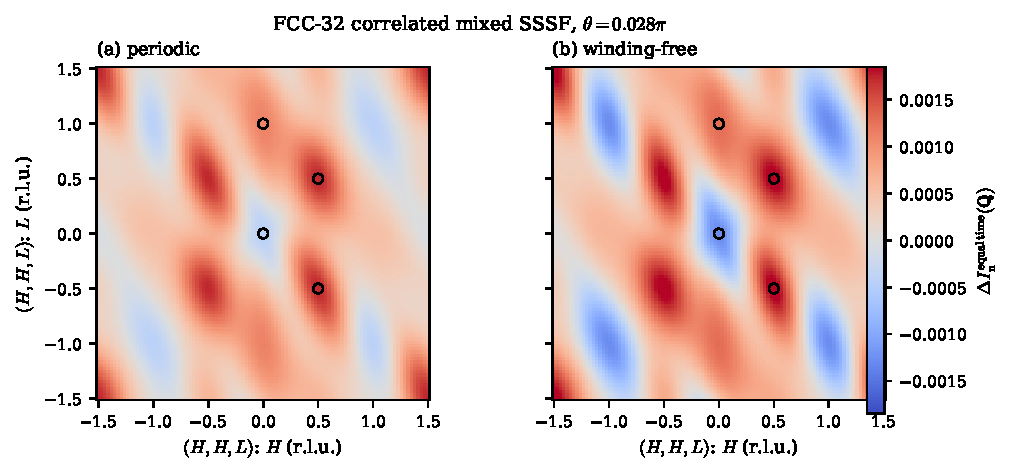
\includegraphics[width=0.88\textwidth]{fig_fcc32_sssf.pdf}
\caption{FCC-32 global unpolarized equal-time structure factor in the
$(H,H,L)$ plane, with the onsite $1/6$ term subtracted. Open circles mark
the representatives in this plane of the eight independent momenta in
Eq.~\eqref{eq:allowedq}. The continuous map is an extended-zone form-factor
evaluation of the finite $32\times32$ correlation matrix, not a continuum of
independent many-body momentum sectors.}
\label{fig:sssf}
\end{figure}

\section{\texorpdfstring{Ce$_2$Hf$_2$O$_7$}{Ce2Hf2O7} constraint}
\label{sec:material}

Smith \emph{et al.} report heat-capacity maxima near $0.065$ and $0.025$ K
and give the seventh-order NLC parameter set A~\cite{Smith2025}
\begin{equation}
 (J_a,J_b,J_c)_A=(0.050,0.021,0.004)\ \mathrm{meV}.
\end{equation}
Taking $J_a$ as the dominant gauge axis and using
Eq.~\eqref{eq:xyzmapSI} gives
\begin{equation}
 \Jzz=0.050\ \mathrm{meV},\qquad
 \Jpm=-0.00625\ \mathrm{meV}.
\end{equation}
Together with Eq.~\eqref{eq:alpha32}, this predicts
$T_{\mathrm{ring}}=7.1$ mK, well below the lower observed feature.

The candidate A$^\star$ in Letter Fig.~4 is defined by three equations,
not by fitting digitized points:
\begin{align}
 \sum_\alpha(J_\alpha^\star)^2&=\sum_\alpha(J_\alpha^A)^2,\\
 J_b^\star-J_c^\star&=J_b^A-J_c^A,\\
 \frac{0.5210289229}{k_B}
 \frac{12|(J_b^\star+J_c^\star)/4|^3}{(J_a^\star)^2}
 &=0.025\ \mathrm{K}.
\end{align}
The solution is
\begin{equation}
 (J_a,J_b,J_c)_{A^\star}=
 (0.0464354,0.0266142,0.0096142)\ \mathrm{meV},
\end{equation}
or $\Jpm^\star=-0.0090571$ meV. The first equation preserves the leading
high-temperature second moment, while the second keeps the transverse
anisotropy of A. These constraints make A$^\star$ a falsifiable target for
a new seventh-order NLC calculation. They do not prove that its complete
high-temperature line shape fits the experiment.

The experimental points and published NLC-A curve in Letter Fig.~4 were
digitized from Fig.~2(a) of Ref.~\cite{Smith2025}, using the source raster and
its logarithmic temperature calibration. They are included only for visual
comparison because the source does not provide tabulated uncertainties. No
likelihood or fit statistic is assigned to those digitized data.

\section{Reproducibility}
\label{sec:repro}

The submission package contains the complete FCC-32 numerical record used in
the Letter:
\begin{itemize}
\item \texttt{scripts/fcc32\_prl\_figures.py} constructs the cluster,
enumerates second- and third-order rows, verifies the mask, diagonalizes the
periodic and projected operators, and generates Letter Figs.~1--4;
\item \texttt{data/fcc32\_prl\_results.npz} contains the spectra,
thermodynamic peaks, allowed momenta, and DSSF arrays;
\item \texttt{data/fcc32\_prl\_results.json} records dimensions, matrix-entry
counts, the exact mask residual, and the A$^\star$ constraints;
\item \path{scripts/digitize_smith2025_heat_capacity.py} documents the
figure calibration used to create
\path{data/ce2hf2o7_smith2025_digitized.csv};
\item \texttt{data/fcc32\_mixed\_sssf.npz} contains the equal-time global
neutron-projection check in Fig.~\ref{fig:sssf}; and
\item \texttt{scripts/recompute\_finite\_size\_artifact.py} is the vendored
FCC geometry, row-enumeration, projection, and thermodynamics module.
\end{itemize}

All frequencies in Letter Fig.~3 are linear, and all of its columns are the
exact FCC-32 momenta listed in Eq.~\eqref{eq:allowedq}. Generated arrays are
stored separately from plotting code to permit direct numerical regression.

\bibliography{references}

\end{document}
